
% l = 8

\begin{figure}[H]
\begin{center}
\subfloat{
\resizebox{8cm}{5cm}{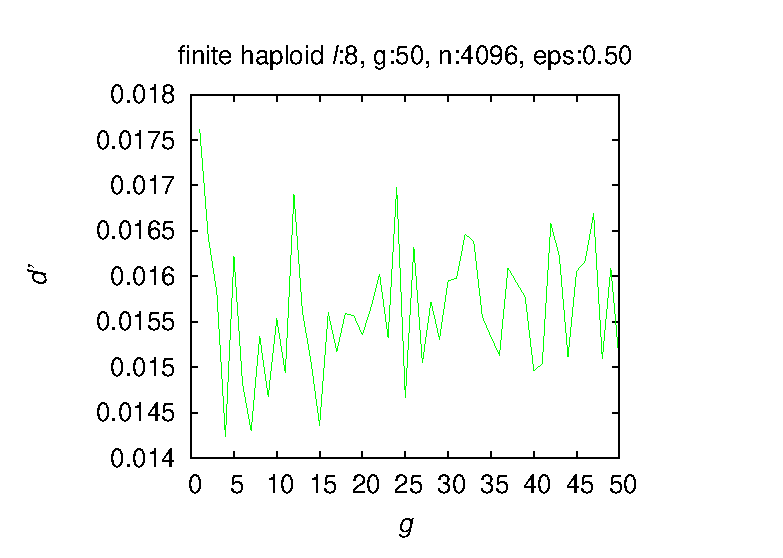
\includegraphics{figures/eps/vio/chi/b8/e0.5/n00004096_fin_hap.eps}}} \hspace{-3em}%
\subfloat{
\resizebox{8cm}{5cm}{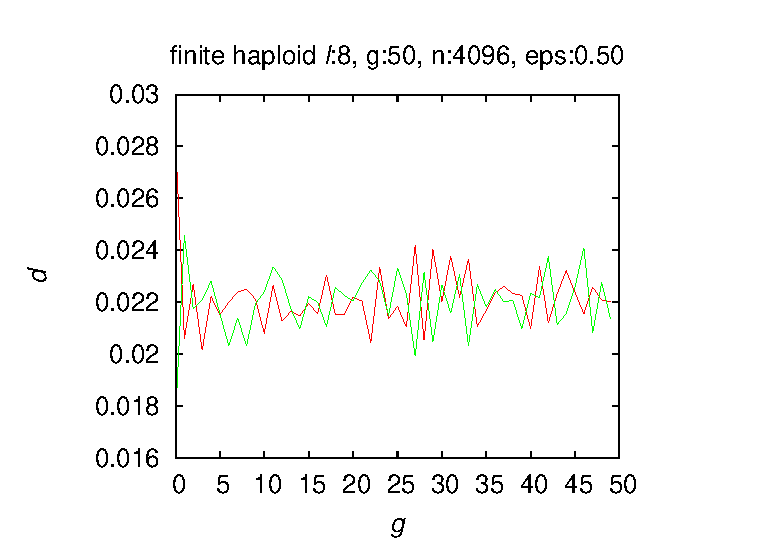
\includegraphics{figures/eps/vio/chi/b8/e0.5/n00004096_fin_hap_wovio.eps}}}\vspace{-1em} \hspace{-3em}%
\end{center}
\begin{center}
\subfloat{
\resizebox{8cm}{5cm}{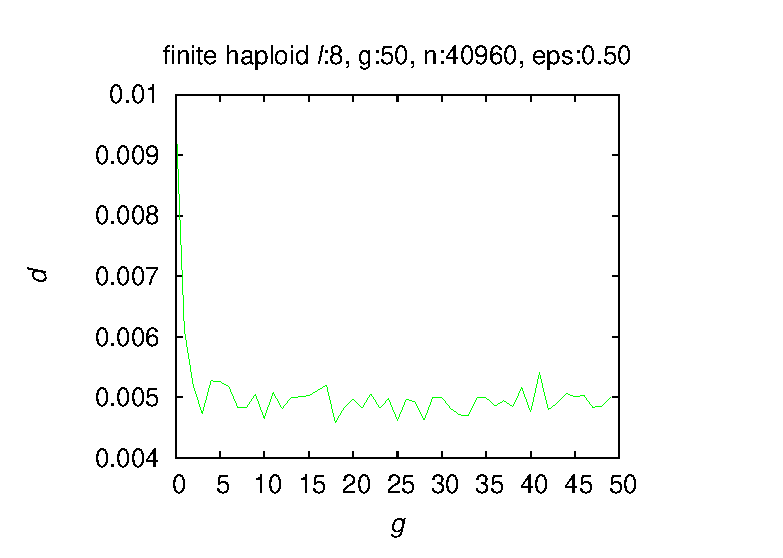
\includegraphics{figures/eps/vio/chi/b8/e0.5/n00040960_fin_hap.eps}}} \hspace{-3em}%
\subfloat{
\resizebox{8cm}{5cm}{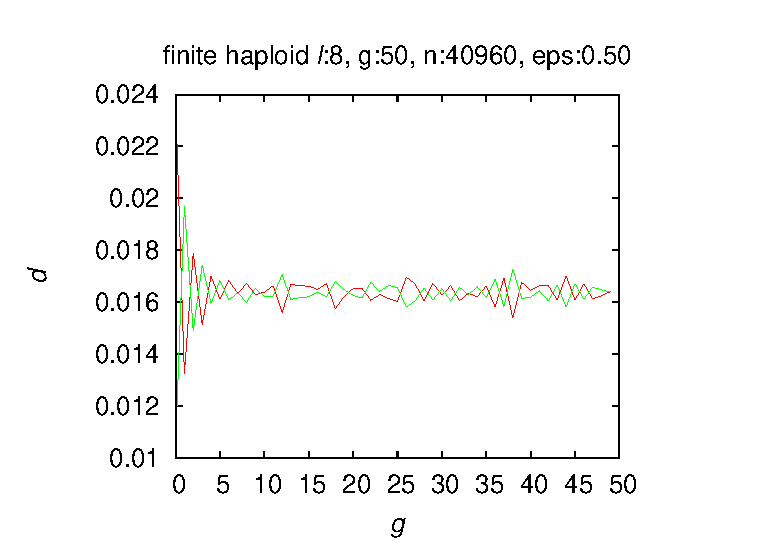
\includegraphics{figures/eps/vio/chi/b8/e0.5/n00040960_fin_hap_wovio.eps}}}\vspace{-1em} \hspace{-3em}%
\end{center}

\begin{center}
\subfloat{
\resizebox{8cm}{5cm}{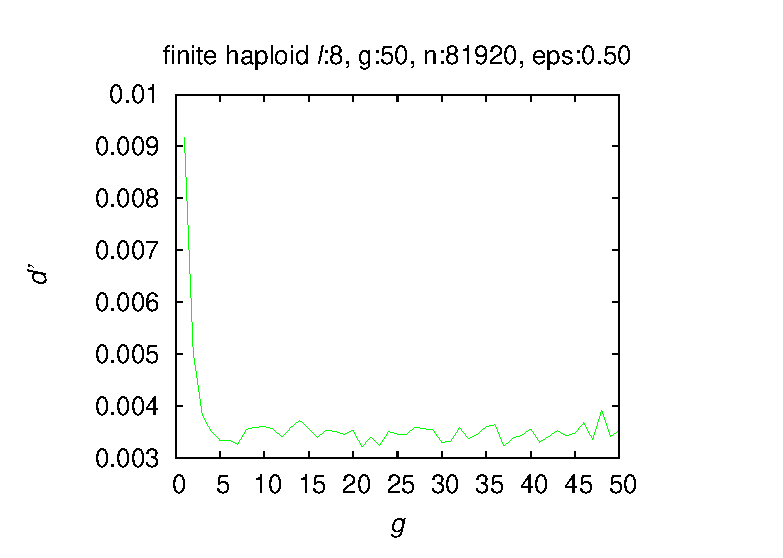
\includegraphics{figures/eps/vio/chi/b8/e0.5/n00081920_fin_hap.eps}}} \hspace{-3em}%
\subfloat{
\resizebox{8cm}{5cm}{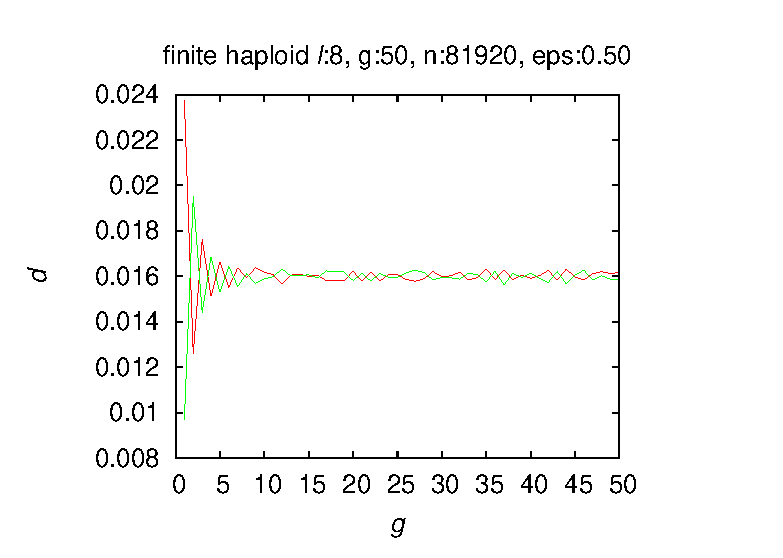
\includegraphics{figures/eps/vio/chi/b8/e0.5/n00081920_fin_hap_wovio.eps}}}\vspace{-1em} \hspace{-3em}%
\end{center}

\begin{center}
\subfloat{
\resizebox{8cm}{5cm}{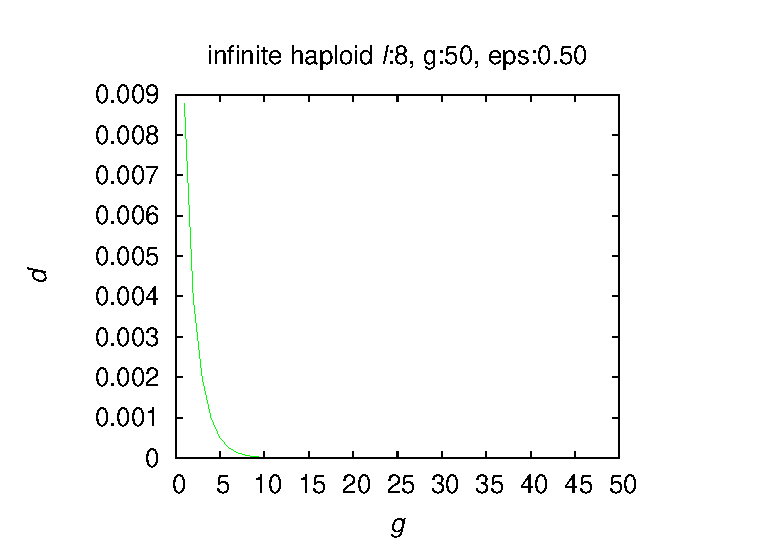
\includegraphics{figures/eps/vio/chi/b8/e0.5/inf_hap.eps}}}\hspace{-3em}%
\subfloat{
\resizebox{8cm}{5cm}{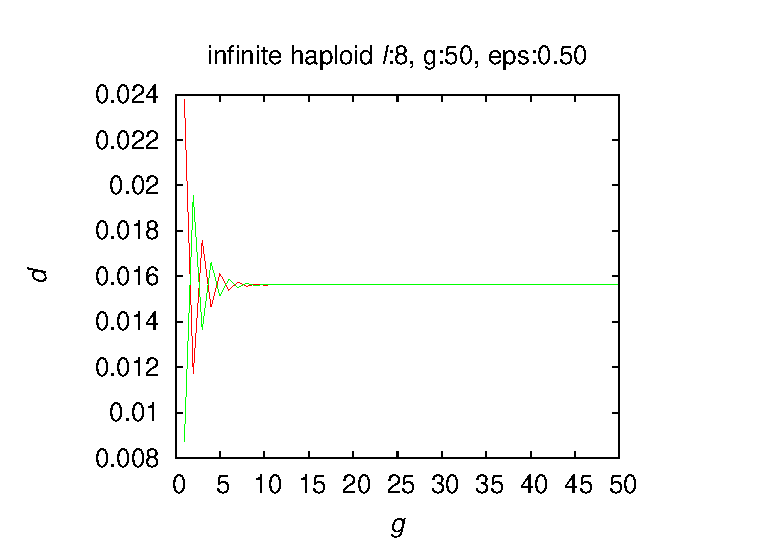
\includegraphics{figures/eps/vio/chi/b8/e0.5/inf_hap_wovio.eps}}}\vspace{-0.5em} \hspace{-3em}%


\caption{\textbf{Infinite and finite haploid population oscillation behavior in case of violation in $\bm{\chi}$ for genome length $\ell = 8$ and $\bm{\epsilon} = 0.5$:} 
  In left column, $d'$ is distance of finite population of size $n$ or infinite population to limit $\bm{z}^\ast$ for $g$ generations. In right column, $d$ is distance of finite population of size $N$ or infinite population to limits without violation.}
\label{oscillation_8h_vio_chi_0.5}
\end{center}
\end{figure}


% l = 10

\begin{figure}[H]
\begin{center}
\subfloat{
\resizebox{8cm}{5cm}{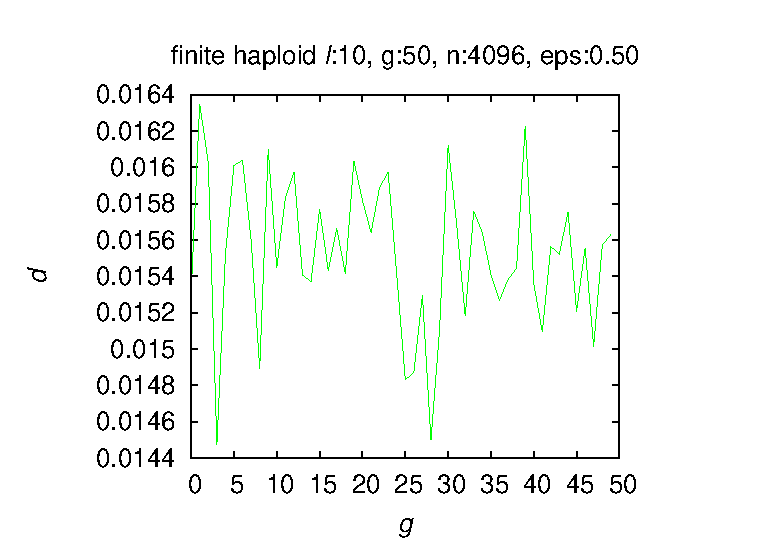
\includegraphics{figures/eps/vio/chi/b10/e0.5/n00004096_fin_hap.eps}}} \hspace{-3em}%
\subfloat{
\resizebox{8cm}{5cm}{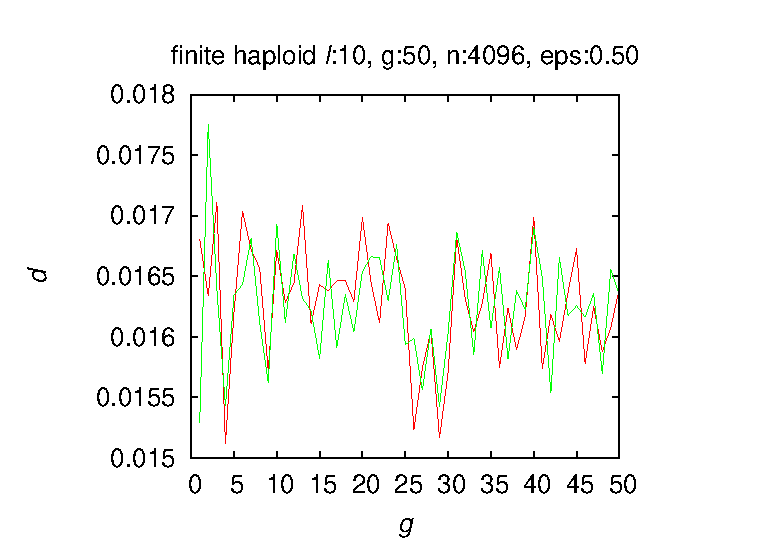
\includegraphics{figures/eps/vio/chi/b10/e0.5/n00004096_fin_hap_wovio.eps}}}\vspace{-1em} \hspace{-3em}%
\end{center}
\begin{center}
\subfloat{
\resizebox{8cm}{5cm}{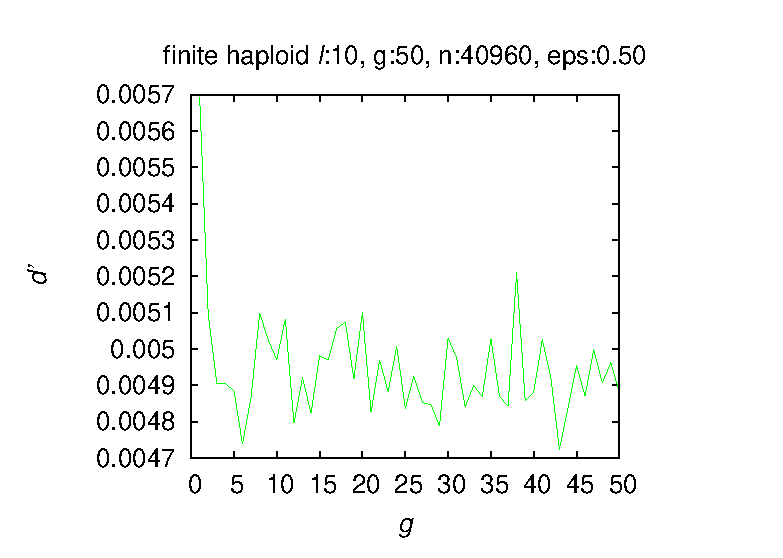
\includegraphics{figures/eps/vio/chi/b10/e0.5/n00040960_fin_hap.eps}}} \hspace{-3em}%
\subfloat{
\resizebox{8cm}{5cm}{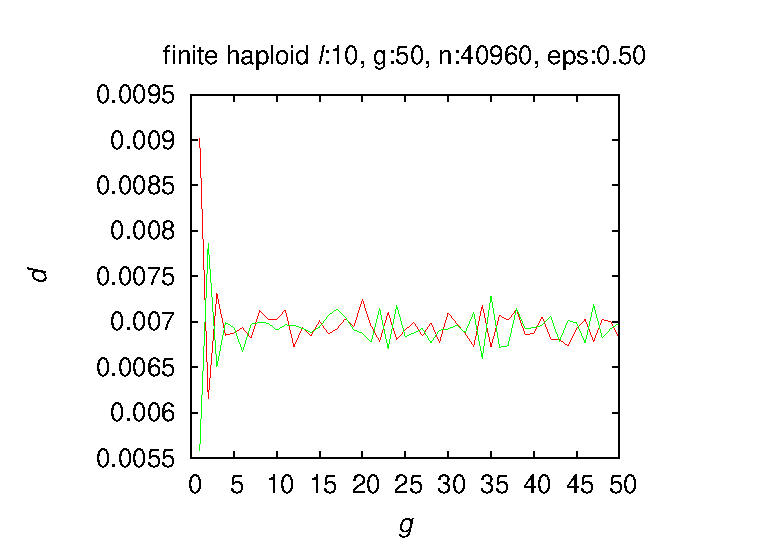
\includegraphics{figures/eps/vio/chi/b10/e0.5/n00040960_fin_hap_wovio.eps}}}\vspace{-1em} \hspace{-3em}%
\end{center}

\begin{center}
\subfloat{
\resizebox{8cm}{5cm}{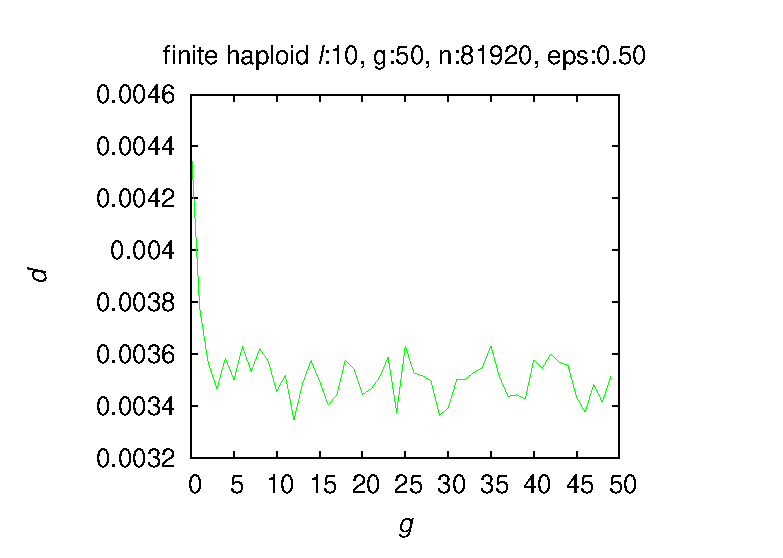
\includegraphics{figures/eps/vio/chi/b10/e0.5/n00081920_fin_hap.eps}}} \hspace{-3em}%
\subfloat{
\resizebox{8cm}{5cm}{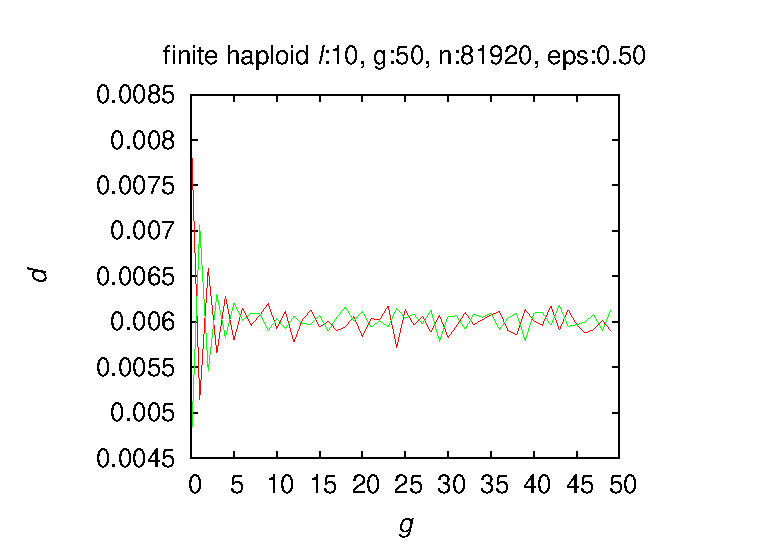
\includegraphics{figures/eps/vio/chi/b10/e0.5/n00081920_fin_hap_wovio.eps}}}\vspace{-1em} \hspace{-3em}%
\end{center}

\begin{center}
\subfloat{
\resizebox{8cm}{5cm}{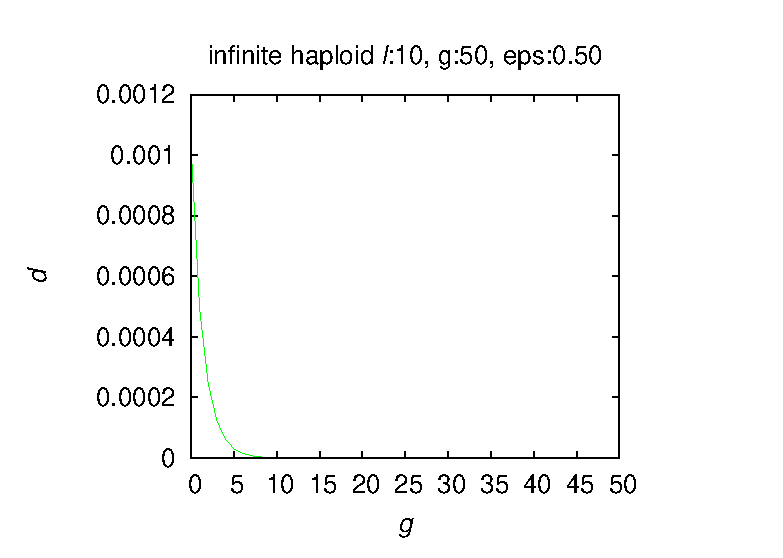
\includegraphics{figures/eps/vio/chi/b10/e0.5/inf_hap.eps}}}\hspace{-3em}%
\subfloat{
\resizebox{8cm}{5cm}{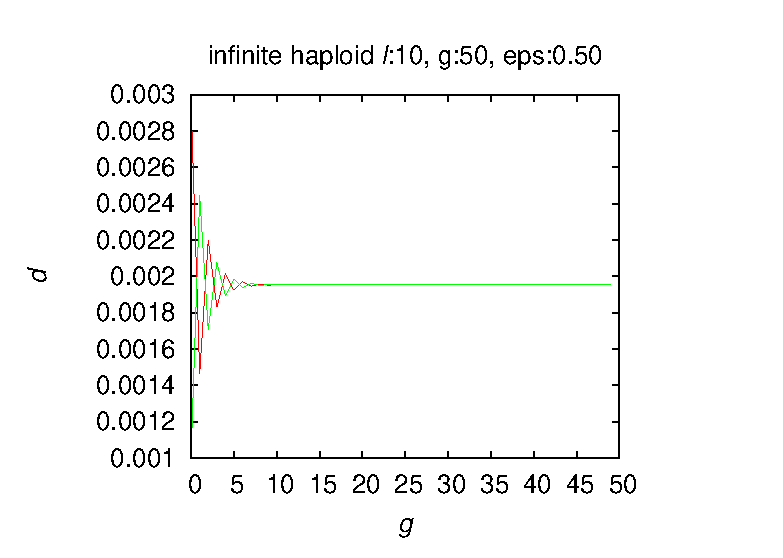
\includegraphics{figures/eps/vio/chi/b10/e0.5/inf_hap_wovio.eps}}}\vspace{-0.5em} \hspace{-3em}%

\caption{\textbf{Infinite and finite haploid population oscillation behavior in case of violation in $\bm{\chi}$ for genome length $\ell = 10$ and $\bm{\epsilon} = 0.5$:} 
  In left column, $d'$ is distance of finite population of size $n$ or infinite population to limit $\bm{z}^\ast$ for $g$ generations. In right column, $d$ is distance of finite population of size $N$ or infinite population to limits without violation.}
\label{oscillation_10h_vio_chi_0.5}
\end{center}
\end{figure}

% l = 12
\begin{figure}[H]
\begin{center}
\subfloat{
\resizebox{8cm}{5cm}{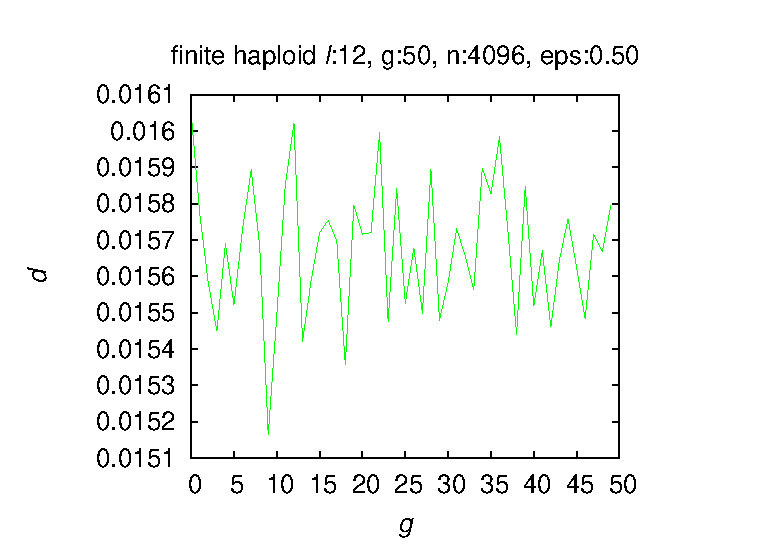
\includegraphics{figures/eps/vio/chi/b12/e0.5/n00004096_fin_hap.eps}}} \hspace{-3em}%
\subfloat{
\resizebox{8cm}{5cm}{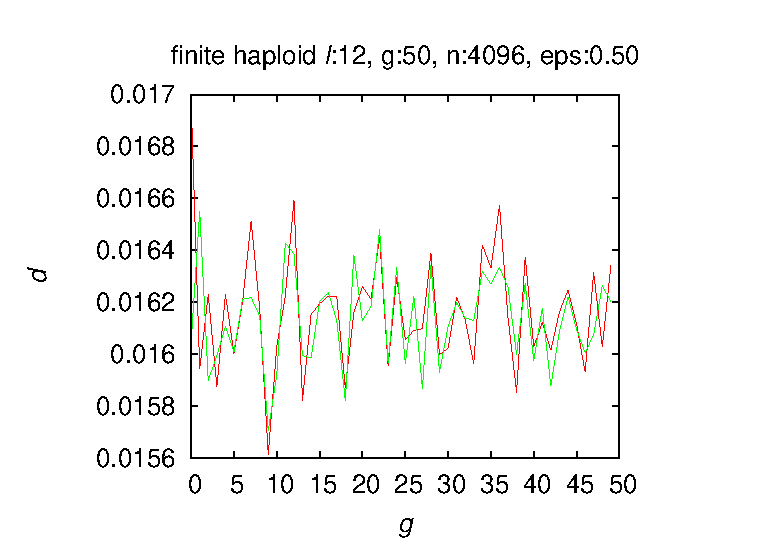
\includegraphics{figures/eps/vio/chi/b12/e0.5/n00004096_fin_hap_wovio.eps}}}\vspace{-1em} \hspace{-3em}%
\end{center}
\begin{center}
\subfloat{
\resizebox{8cm}{5cm}{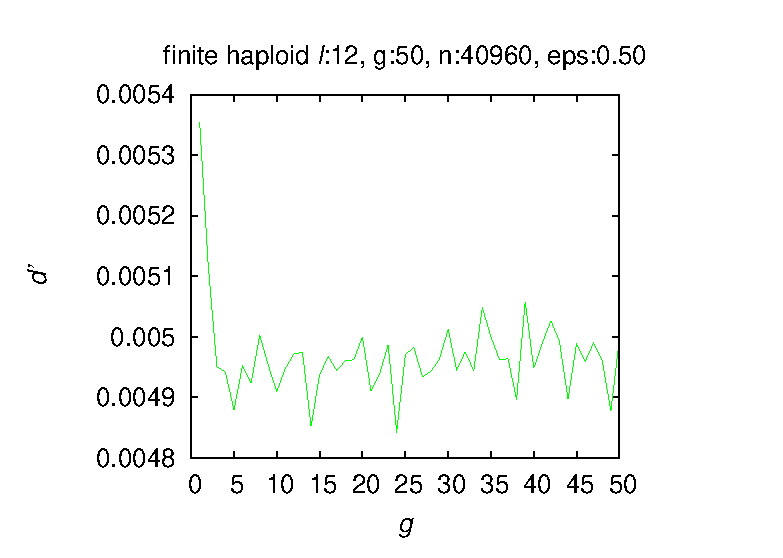
\includegraphics{figures/eps/vio/chi/b12/e0.5/n00040960_fin_hap.eps}}} \hspace{-3em}%
\subfloat{
\resizebox{8cm}{5cm}{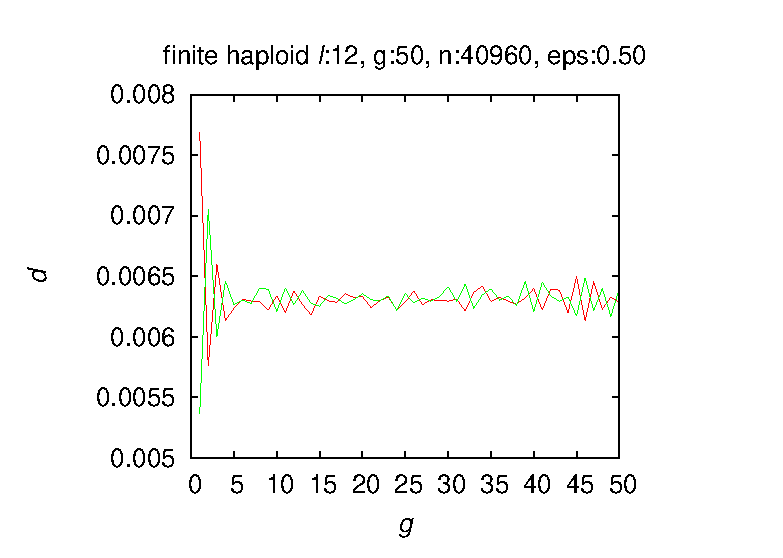
\includegraphics{figures/eps/vio/chi/b12/e0.5/n00040960_fin_hap_wovio.eps}}}\vspace{-1em} \hspace{-3em}%
\end{center}

\begin{center}
\subfloat{
\resizebox{8cm}{5cm}{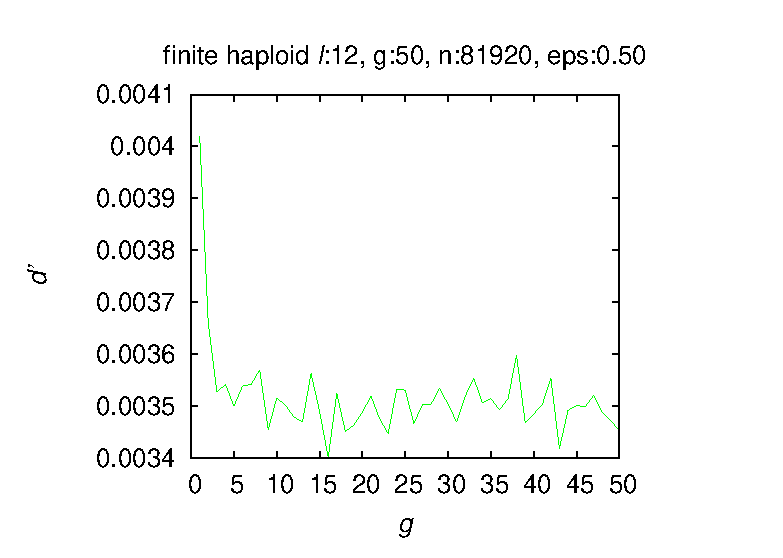
\includegraphics{figures/eps/vio/chi/b12/e0.5/n00081920_fin_hap.eps}}} \hspace{-3em}%
\subfloat{
\resizebox{8cm}{5cm}{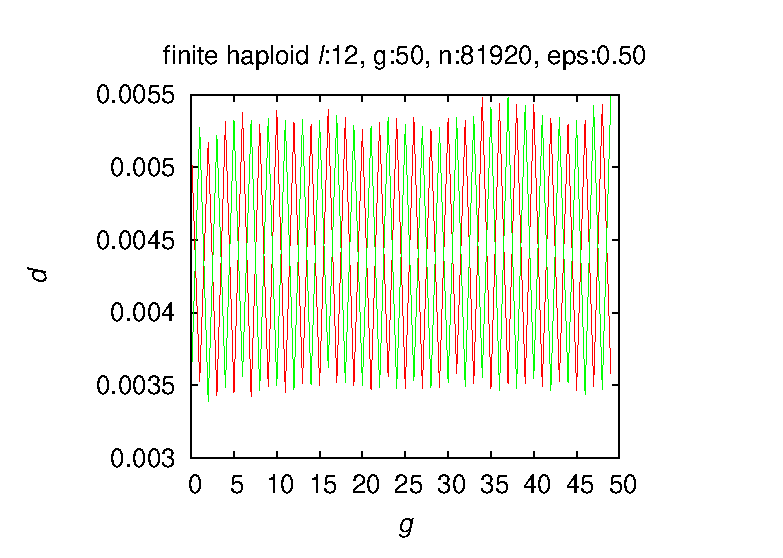
\includegraphics{figures/eps/vio/chi/b12/e0.5/n00081920_fin_hap_wovio.eps}}}\vspace{-1em} \hspace{-3em}%
\end{center}

\begin{center}
\subfloat{
\resizebox{8cm}{5cm}{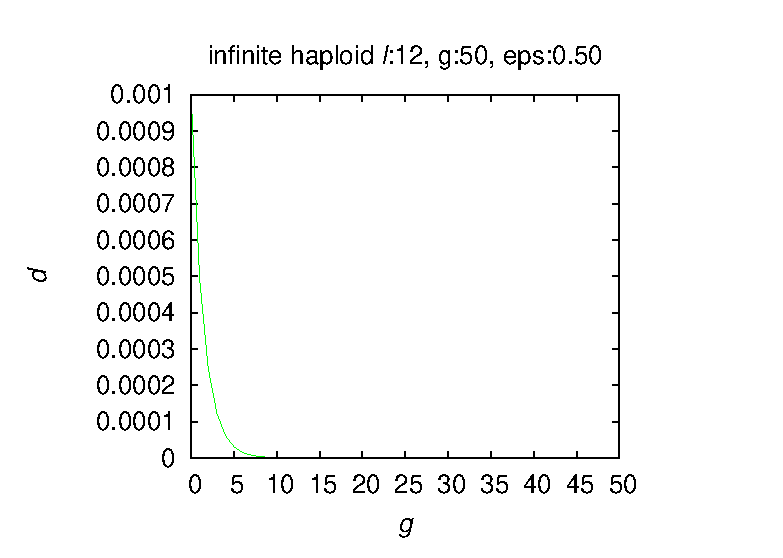
\includegraphics{figures/eps/vio/chi/b12/e0.5/inf_hap.eps}}}\hspace{-3em}%
\subfloat{
\resizebox{8cm}{5cm}{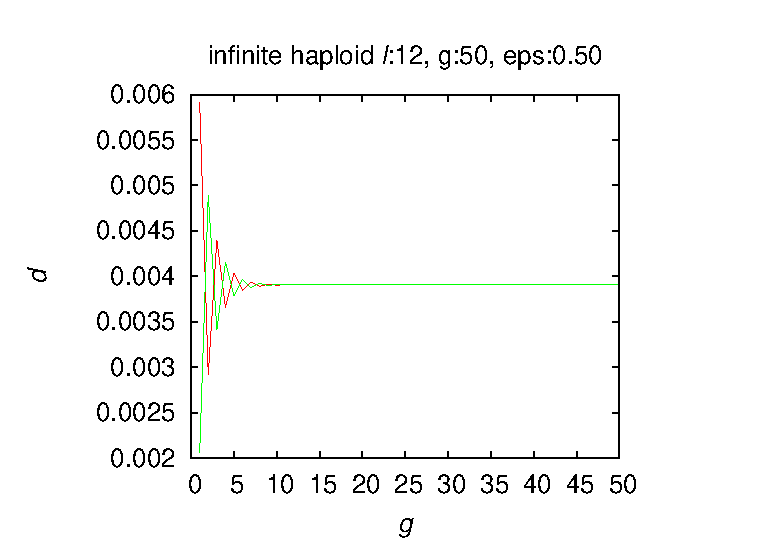
\includegraphics{figures/eps/vio/chi/b12/e0.5/inf_hap_wovio.eps}}}\vspace{-0.5em} \hspace{-3em}%


\caption{\textbf{Infinite and finite haploid population oscillation behavior in case of violation in $\bm{\chi}$ for genome length $\ell = 12$ and $\bm{\epsilon} = 0.5$:} 
  In left column, $d'$ is distance of finite population of size $n$ or infinite population to limit $\bm{z}^\ast$ for $g$ generations. In right column, $d$ is distance of finite population of size $N$ or infinite population to limits without violation.}
\label{oscillation_12h_vio_chi_0.5}
\end{center}
\end{figure}

% l = 14

\begin{figure}[H]
\begin{center}
\subfloat{
\resizebox{8cm}{5cm}{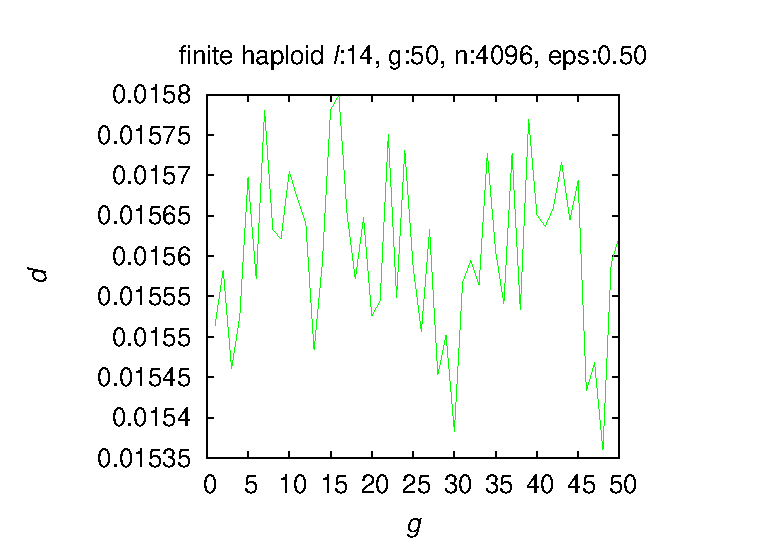
\includegraphics{figures/eps/vio/chi/b14/e0.5/n00004096_fin_hap.eps}}} \hspace{-3em}%
\subfloat{
\resizebox{8cm}{5cm}{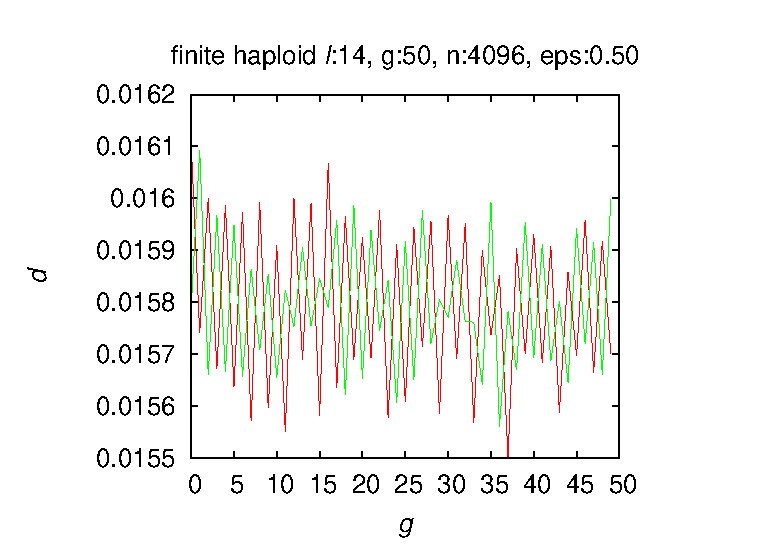
\includegraphics{figures/eps/vio/chi/b14/e0.5/n00004096_fin_hap_wovio.eps}}}\vspace{-1em} \hspace{-3em}%
\end{center}
\begin{center}
\subfloat{
\resizebox{8cm}{5cm}{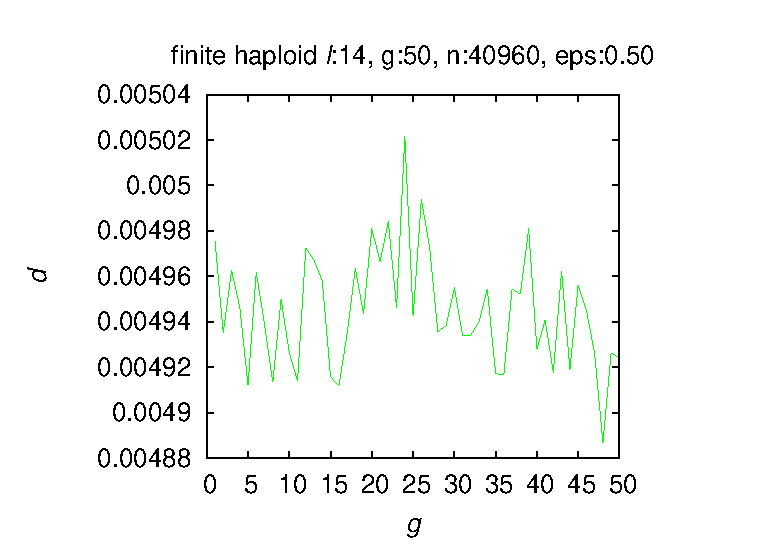
\includegraphics{figures/eps/vio/chi/b14/e0.5/n00040960_fin_hap.eps}}} \hspace{-3em}%
\subfloat{
\resizebox{8cm}{5cm}{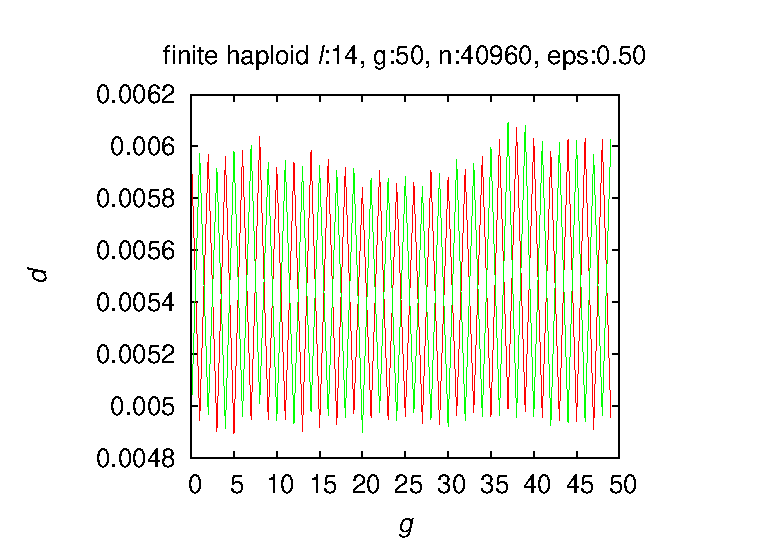
\includegraphics{figures/eps/vio/chi/b14/e0.5/n00040960_fin_hap_wovio.eps}}}\vspace{-1em} \hspace{-3em}%
\end{center}

\begin{center}
\subfloat{
\resizebox{8cm}{5cm}{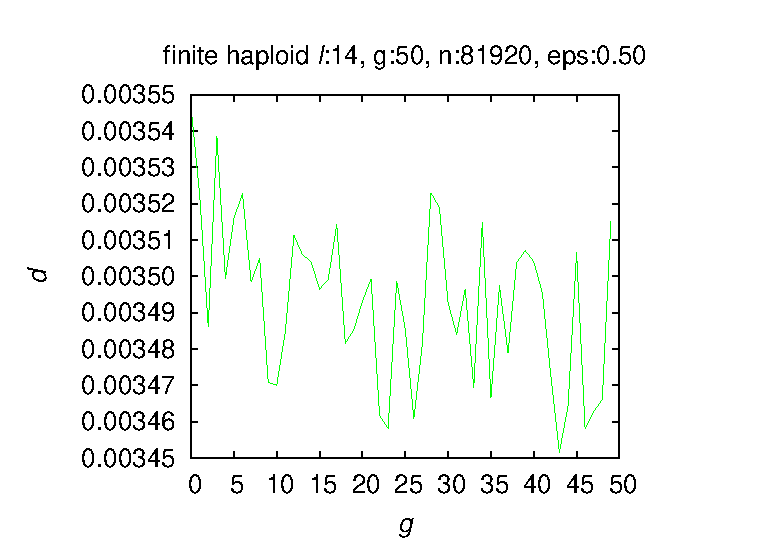
\includegraphics{figures/eps/vio/chi/b14/e0.5/n00081920_fin_hap.eps}}} \hspace{-3em}%
\subfloat{
\resizebox{8cm}{5cm}{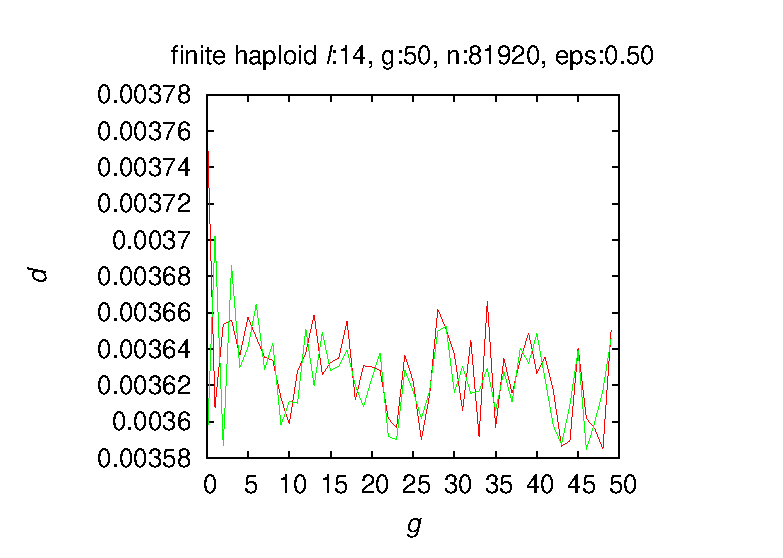
\includegraphics{figures/eps/vio/chi/b14/e0.5/n00081920_fin_hap_wovio.eps}}}\vspace{-1em} \hspace{-3em}%
\end{center}

\begin{center}
\subfloat{
\resizebox{8cm}{5cm}{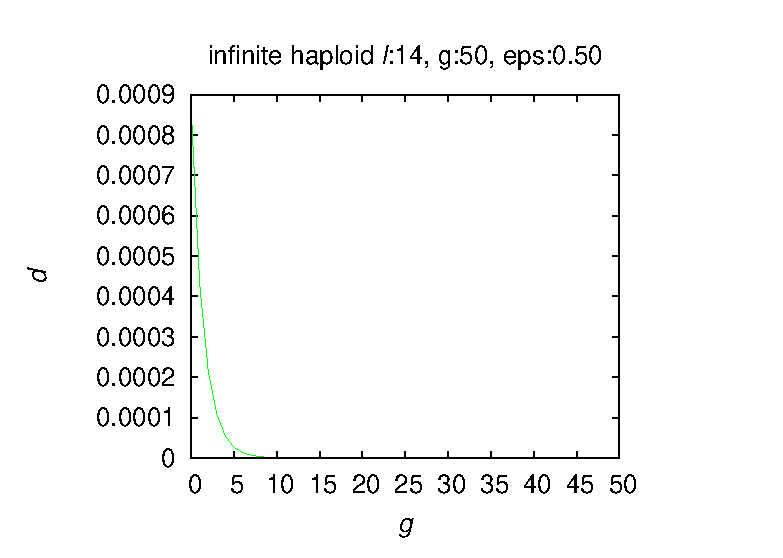
\includegraphics{figures/eps/vio/chi/b14/e0.5/inf_hap.eps}}}\hspace{-3em}%
\subfloat{
\resizebox{8cm}{5cm}{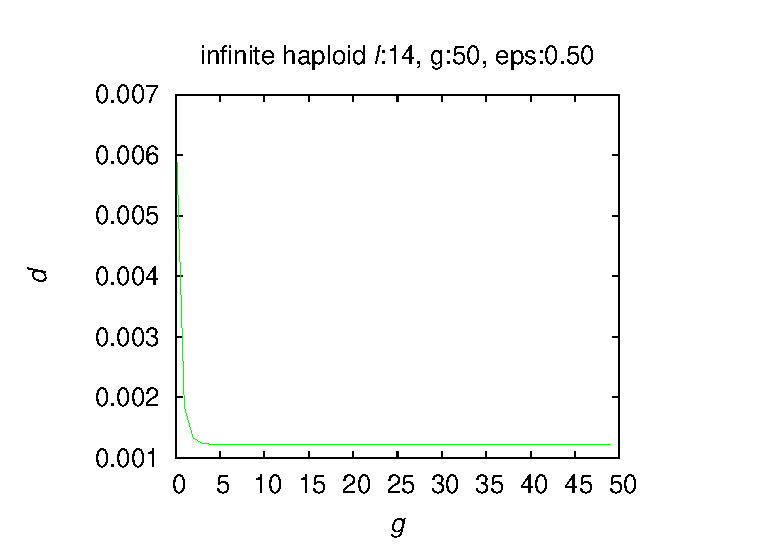
\includegraphics{figures/eps/vio/chi/b14/e0.5/inf_hap_wovio.eps}}}\vspace{-0.5em} \hspace{-3em}%

\caption{\textbf{Infinite and finite haploid population oscillation behavior in case of violation in $\bm{\chi}$ for genome length $\ell = 14$ and $\bm{\epsilon} = 0.5$:} 
  In left column, $d'$ is distance of finite population of size $n$ or infinite population to limit $\bm{z}^\ast$ for $g$ generations. In right column, $d$ is distance of finite population of size $N$ or infinite population to limits without violation.}
\label{oscillation_14h_vio_chi_0.5}
\end{center}
\end{figure}

The right column in figures \ref{oscillation_8h_vio_chi_0.5} through \ref{oscillation_14h_vio_chi_0.5} 
shows distance of finite and infinite haploid populations to non-violation limits $\bm{p^\ast}$ and $\bm{q^\ast}$ with $\bm{\epsilon} \;=\; 0.5$. 
Graphs in the right column give picture of oscillating behavior of haploid population given violation. 
Unlike in case of mutation distribution with violation with $\bm{\epsilon} \;=\; 0.5$, absence of oscillation was not observed. 
Finite populations still oscillate, and infinite populations aslo oscillate but dies out completely quickly. 
Dying out of oscillation in infinite population is quicker than when $\bm{\epsilon} \;=\; 0.1$ for violation in $\bm{chi}$ in haploid case. 

The left column of figures \ref{oscillation_8h_vio_chi_0.5} through \ref{oscillation_14h_vio_chi_0.5} 
shows distance of finite and infinite haploid populations to limit $\bm{z^\ast}$ 
(limit with violation in crossover distribution $\bm{\chi}$) when $\bm{\epsilon} \;=\; 0.5$. 
The distance between finite population and limit $\bm{z}^\ast$ (limit with violation in $\bm{\chi}$ distribution) 
decreases as finite population size increases, 
and finite population shows behavior similar to infinite population behavior as finite population reach large number. 
The distance data for haploid population in case of violation in $\bm{\chi}$ distribution 
with $\bm{\epsilon} \;=\; 0.5$ for different finite population size $N$ are tabulated in table \ref{distanceChiHapEps0.5}. 

\begin{table}[ht]
\caption{\textbf{Distance measured for violation in $\bm{\chi}$ with $\bm{\epsilon} \;=\; 0.5$  for haploids:} $\ell$ is genome length, 
and average distance between finite and 
infinite populations is tabulated in last three columns.}
\centering
\begin{tabularx}{0.75\textwidth}{ c *{3}{X}}
\toprule
$\ell$ & $N = 4096$ & $N = 40960$ & $N = 81920$  \\
\midrule
8 & 0.0156	&  0.0051	& 0.0036 \\
10 & 0.0155	&  0.0049	& 0.0035 \\
12 & 0.0157	&  0.0050	& 0.0035 \\
14 & 0.0156	&  0.0049	& 0.0035 \\      
\bottomrule
\end{tabularx}
\label{distanceChiHapEps0.5}
\end{table} 

From table \ref{distanceChiHapEps0.5}, average distance calculated for finite population size $4096$ is $0.0156$, 
for size $40960$ is $0.0050$ and for size $81920$ is $0.0035$. These results show average distance 
between finite population and limit $\bm{z^\ast}$ closely follows expected single step distance 
between finite and infinite population given in \ref{tableExpectedDistance}. The distance decreased as $1/\sqrt{N}$. 








